\documentclass[10pt, xcolor=x11names, compress]{beamer}
%\documentclass[10pt, xcolor=x11names, compress, handout]{beamer}
\usetheme{progressbar}
%\usecolortheme[named=Purple4]{structure}
\progressbaroptions{headline=sections,titlepage=normal,frametitle=normal}

\setbeamertemplate{navigation symbols}{}

\usepackage{iwona} 

\usepackage{alltt}
\usepackage{amsmath,amsfonts, amssymb, amscd}
\usepackage{hyperref}
\usepackage{setspace}
\usepackage{wasysym}
\usepackage{ulem}

\usepackage{calc}
\usepackage[overlay,absolute]{textpos}
\TPGrid[5mm,5mm]{20}{20}



\renewcommand{\Re}{\operatorname{Re}}
\renewcommand{\Im}{\operatorname{Im}}
\newcommand{\debye}{\operatorname{debye}}

\newcommand{\chik}{$\chi(k)$}
\newcommand{\chir}{$|\tilde{\chi}(R)|$}


\newcommand{\file}[1]{{\color{Firebrick4}\texttt{`#1'}}}
\newcommand{\multiple}{{\color{Orange3}\textsl{multiple}}}


\newcommand{\atoms}  {{\color{DarkOrchid4}\textsc{atoms}}}
\newcommand{\feff}   {{\color{DarkOrchid4}\textsc{feff}}}
\newcommand{\ifeffit}{{\color{DarkOrchid4}\textsc{ifeffit}}}
\newcommand{\athena} {{\color{DarkOrchid4}\textsc{athena}}}
\newcommand{\artemis}{{\color{DarkOrchid4}\textsc{artemis}}}

\renewenvironment<>{center}
{\begin{actionenv}#1\begin{originalcenter}}
{\end{originalcenter}\end{actionenv}}

\definecolor{guessp}   {rgb}{0.64,0.00,0.64}
\newcommand{\guessp}   {{\color{guessp}guess}}
\definecolor{defp}     {rgb}{0.00,0.55,0.00}
\newcommand{\defp}     {{\color{defp}def}}
\definecolor{setp}     {rgb}{0,0,0}
\newcommand{\setp}     {{\color{setp}set}}
\definecolor{lguessp}  {rgb}{0.24,0.11,0.56}
\newcommand{\lguessp}  {{\color{lguessp}lguess}}
\definecolor{skipp}    {rgb}{0.70,0.70,0.70}
\newcommand{\skipp}    {{\color{skipp}skip}}
\definecolor{restrainp}{rgb}{0.80,0.61,0.11}
\newcommand{\restrainp}{{\color{restrainp}restrain}}
\definecolor{afterp}   {rgb}{0.29,0.44,0.55}
\newcommand{\afterp}   {{\color{afterp}after}}
\definecolor{penaltyp} {rgb}{0.55,0.35,0.17}
\newcommand{\penaltyp} {{\color{penaltyp}penalty}}
\definecolor{mergep}   {rgb}{0.93,0.00,0.00}
\newcommand{\mergep}   {{\color{mergep}merge}}


%% define new commands here
%\newcommand{\eto}{EuTiO$_3$}

\mode<presentation>

\title{The Ramsauer-Townsend effect in EXAFS}
%\subtitle{}

\author{Bruce Ravel}
\institute[NIST]{Synchrotron Methods Group, Materials Measurement Science Division\\%
  Materials Measurement Laboratory\\%
  National Institute of Standards and Technology\\%
  \&\\%
  Local Contact, Beamline X23A2\\%
  National Synchrotron Light Source\\~}


\date{\today}

\begin{document}
\maketitle

\begin{frame}
  \frametitle{Copyright}
  \tiny

  This document is copyright \copyright 2007-2010 Bruce Ravel.

  \begin{center}
    
\includegraphics[width=1.0cm]{images/somerights20}
  \end{center}

  This work is licensed under the Creative Commons
  Attribution-ShareAlike License.  To view a copy of this license,
  visit \href{http://creativecommons.org/licenses/by-sa/3.0/}
  {\color{Purple4}\texttt{http://creativecommons.org/licenses/by-sa/3.0/}}
  or send a letter to Creative Commons, 559 Nathan Abbott Way,
  Stanford, California 94305, USA.

  \begin{description}
  \item[You are free:] %
    \begin{itemize}
    \item \textbf{to Share} --- to copy, distribute, and transmit the work
    \item \textbf{to Remix} --- to adapt the work
    \end{itemize}
  \item[Under the following conditions:] %
    \begin{itemize}
    \item Attribution. You must attribute the work in the manner
      specified by the author or licensor (but not in any way that
      suggests that they endorse you or your use of the work).
    \item Share Alike. If you alter, transform, or build upon this
      work, you may distribute the resulting work only under the same,
      similar or a compatible license.
    \item Any of these conditions can be waived if you get permission
      from the author.
    \end{itemize}
  \end{description}
  \begin{itemize}
  \item For any reuse or distribution, you must make clear to others
    the license terms of this work. The best way to do this is with a
    link to the URL for this document.
  \item Any of the above conditions can be waived if you get
    permission from the copyright holder.
  \item Nothing in this license impairs or restricts the author's
    moral rights.
  \end{itemize}

  Your fair dealing and other rights are in no way affected by the
  above.  This is a human-readable summary of the Legal Code (the full
  license).


\end{frame}

%%% Local Variables:
%%% mode: latex
%%% TeX-master: "pimst2"
%%% End:


\begin{frame}
  \frametitle{Here's a beginner's question}

  \begin{columns}[T]
    \begin{column}{0.5\linewidth}
      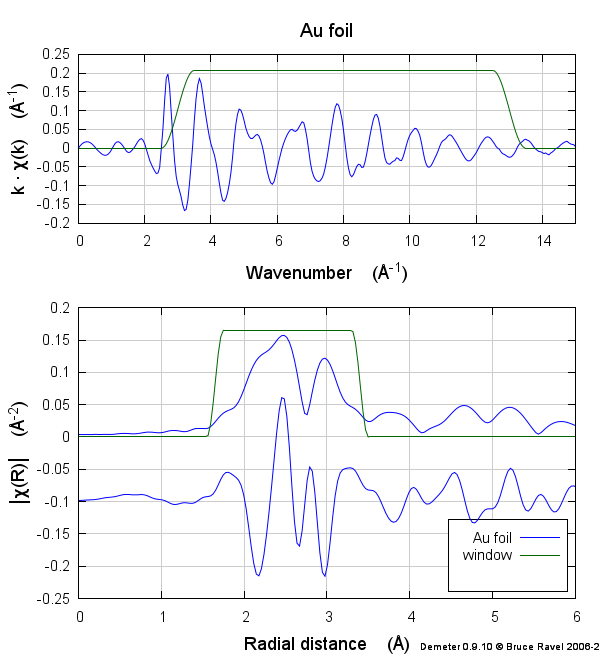
\includegraphics[width=\linewidth]{Au_rk.png}
    \end{column}
    \begin{column}{0.5\linewidth}
      Here are data on a gold foil.  Gold is an FCC metal with 12
      neighbors in the first coordination shell at $\sim2.9$\,\AA\
      and 6 in the second shell at $\sim4.1$\,\AA.

      \bigskip

      The Fourier transform of these data -- done with k-weight = 1 in
      order to emphasize the point -- clearly show a split peak in the
      $|\tilde\chi(R)|$ spectrum with peaks at about 2.5\,\AA\ and
      3.0\,\AA.

      \bigskip

      \begin{alertblock}{}
        \centering How can this be?
      \end{alertblock}
    \end{column}
  \end{columns}
\end{frame}

\begin{frame}
  \frametitle{Sum of sine waves}
  Here is an overly simplified representation of the EXAFS signal
  using pure, undamped sine waves.

  \bigskip

  \begin{columns}
    \begin{column}{0.5\linewidth}
      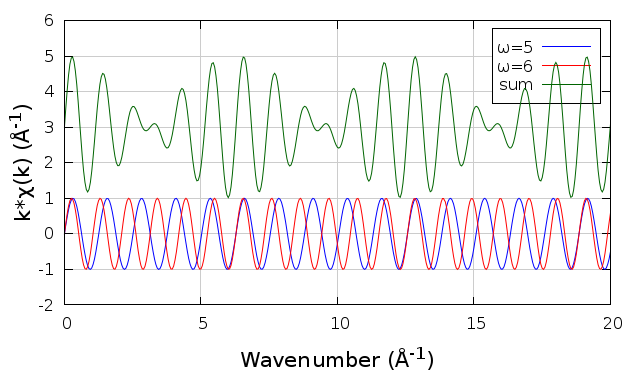
\includegraphics[width=\linewidth]{beat_k.png}
    \end{column}
    \begin{column}{0.5\linewidth}
      The {\color{Blue2}blue} wave has a frequency of 5, representing a
      distance of 2.5\,\AA.

      \medskip

      The {\color{Red2}red} wave has a frequency of 6, representing a
      distance of 3\,\AA.

      \medskip

      The {\color{Green4}green} wave is the sum of those two.  This
      summation results in a beating pattern.
    \end{column}
  \end{columns}
\end{frame}


\begin{frame}
  \frametitle{The Fourier transform of the sum}
  Here I show an EXAFS-like, finite-range Fourier transform over $2k$.
  The k-range was 3\,\AA\ -- 16\,\AA, the window sill was 1\,\AA, and
  a Kaiser-Bessel window was used.

  \bigskip

  \begin{columns}
    \begin{column}{0.5\linewidth}
      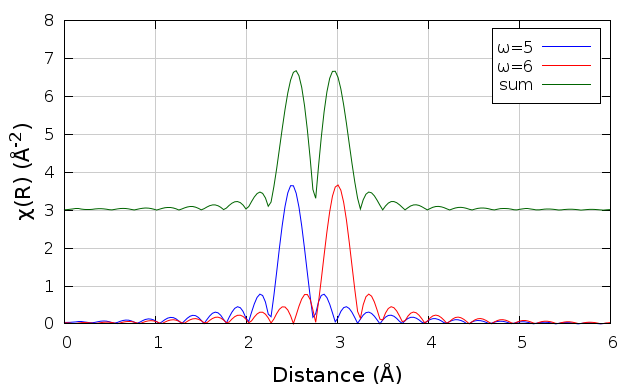
\includegraphics[width=\linewidth]{beat_r.png}
    \end{column}
    \begin{column}{0.5\linewidth}
      The {\color{Blue2}blue} and {\color{Red2}red} waves have peaks
      at 2.5\,\AA\ and 3\,\AA, as expected.

      \medskip
      
      The Fourier transform of the sum, the {\color{Green4}green}
      wave, has peaks at both 2.5\,\AA\ and at 3\,\AA.
    \end{column}
  \end{columns}
\end{frame}

\begin{frame}
  \frametitle{Interpreting the Au foil data}
  \begin{columns}
    \begin{column}{0.5\linewidth}
      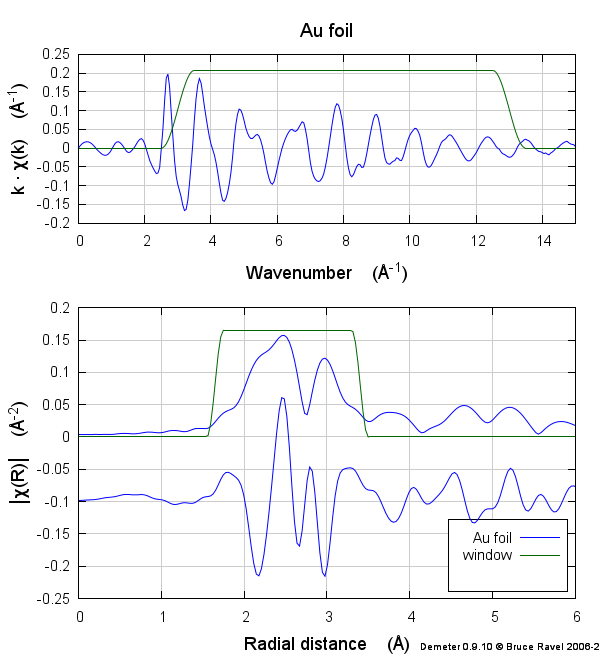
\includegraphics[width=\linewidth]{Au_rk.png}      
    \end{column}
    \begin{column}{0.5\linewidth}
      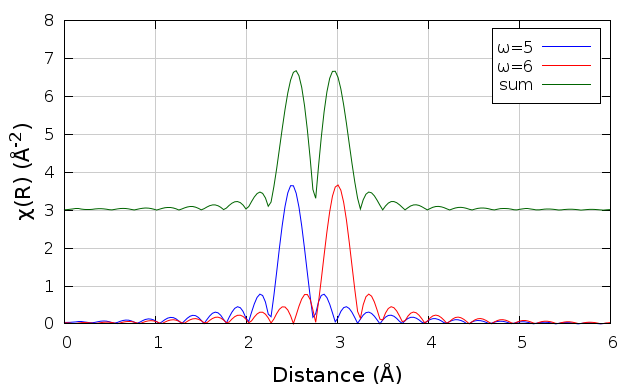
\includegraphics[width=\linewidth]{beat_r.png}

      \medskip

      Does this mean that we actually have 2 near-neighbor distances
      in our gold foil?
    \end{column}
  \end{columns}
  \begin{alertblock}<2>{}
    \centering Certainly not!
  \end{alertblock}
\end{frame}

\begin{frame}
  \frametitle{The EXAFS Equation}
  {\small
    \begin{align}
      \chi(k,\Gamma) =&
      { \frac{{\color{SlateBlue3}(N_\Gamma S_0^2)}{\color{Gold4}F_\Gamma(k)}}
        {2\,kR_\Gamma^2} }
      \sin(2kR_\Gamma + {\color{Gold4}\Phi_\Gamma(k)})
      e^{-2{\color{SlateBlue3}\sigma_\Gamma^2}k^2}
      e^{-2R_\Gamma/{\color{Gold4}\lambda(k)}} \\
      \chi_{\mathrm{theory}}(k) =& \sum\limits_{\Gamma}\chi(k,\Gamma) \notag\\
      R_\Gamma =& \> {\color{Gold4}R_{0,\Gamma}} +
      {\color{SlateBlue3}\Delta R_\Gamma} \\
      k =& N\sqrt{(E_0 - {\color{SlateBlue3}\Delta E_0})}
    \end{align}}

  \medskip

  It is certainly true that we sum up terms with $\sin(2kR_\Gamma)$
  (like in our simple, sine-wave example), however we also have the
  terms ${\color{Gold4}F_\Gamma(k)}$ and
  ${\color{Gold4}\Phi_\Gamma(k)}$ in the EXAFS equation.

  \medskip

  \begin{block}{}
    \centering What does ${\color{Gold4}F_\Gamma(k)}$ look like for
    something as heavy as Au?
  \end{block}
\end{frame}

\begin{frame}
  \frametitle{The scattering amplitude}
  Here is ${\color{Gold4}F_\Gamma(k)}$. as calculated by {\feff} for
  the first shell Au atom in FCC gold.
  \begin{center}
    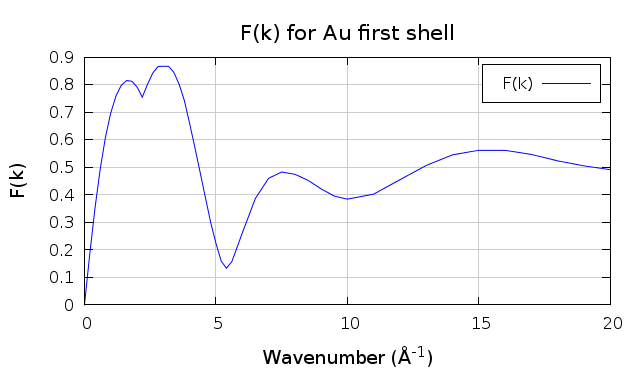
\includegraphics[width=0.7\linewidth]{f_au.png}
  \end{center}
  The minimum just above 5\,\AA\ will introduce structure to the EXAFS
  equation that resembles the beat due to the sum of sine waves.
  \begin{textblock*}{0.7\linewidth}(0pt,19.5\TPVertModule)%
    \tiny%
    Here I am plotting columns 1 v.\ 3 from the file \file{feff0001.dat}.
  \end{textblock*}
\end{frame}

\begin{frame}
  \frametitle{Simple model from quantum scattering theory}
  The basic physics of this phenomenon is related to the well-known
  problem of scattering from a square potential.  All first-year
  physics graduate students have to solve the 1D problem of scattering
  from a square potential.
  \begin{columns}[T]
    \begin{column}{0.6\linewidth}
      \centering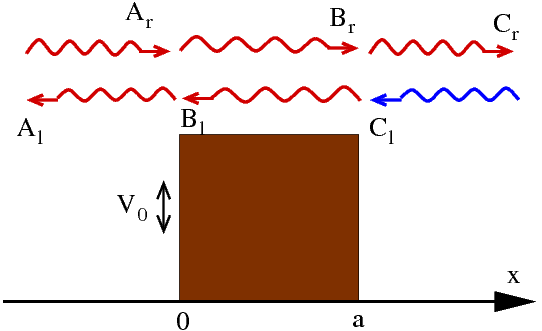
\includegraphics[width=0.7\linewidth]{Finitepot.png}
    \end{column}
    \begin{column}{0.4\linewidth}
      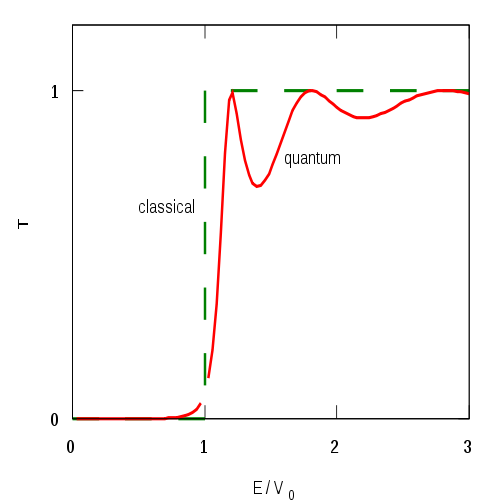
\includegraphics[width=0.7\linewidth]{Finitebarrdiag.png}      
    \end{column}
  \end{columns}
  In the quantum problem, there is a large tunneling probability at
  certain enegies (wavelengths).  At the minimum in
  ${\color{Gold4}F_\Gamma(k)}$, we are seeing tranmission of the
  photoelectron through the scatterer.
  \begin{textblock*}{0.7\linewidth}(0pt,19.5\TPVertModule)%
    \tiny%
    These images from Wikimedia Commons.\\See
    \href{http://en.wikipedia.org/wiki/Rectangular_potential_barrier}
    {\color{Blue2}the Wikipedia ``Rectangular potential barrier'' page}
  \end{textblock*}
\end{frame}

\begin{frame}
  \frametitle{Feff's calculation of the first shell in Au}
  \begin{columns}
    \begin{column}{0.5\linewidth}
      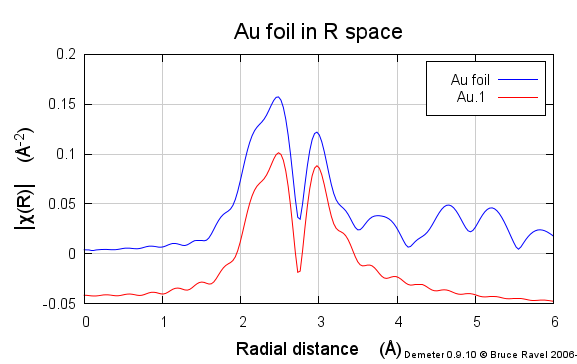
\includegraphics[width=\linewidth]{Au+path.png}
    \end{column}
    \begin{column}{0.5\linewidth}
      {\feff} accounts for the Ramsauer-Townsend effect correctly in
      its calculation, enabling analysis in the same manner as for
      lighter elements.

      \bigskip

      One moral of this story is that it is always wise to compare a
      {\feff} calculation with your data before jumping to conclusions
      about the interpetation of the peaks in $\tilde\chi(R)$.
    \end{column}
  \end{columns}

  \bigskip

  \begin{alertblock}{$\tilde\chi(R)$ is \textbf{NOT} a radial distribution function!}
    The Ramsauer-Townsend effect on ${\color{Gold4}F_\Gamma(k)}$ is
    among the many reasons $\tilde\chi(R)$ is \textbf{NOT} an RDF.
  \end{alertblock}
\end{frame}

\begin{frame}
  \frametitle{Bibliography}
  \small%
  Searching for ``Ramsauer Townsend EXAFS'' on Google Scholar turns up
  dozens of examples of papers discussing this phenomenon in EXAFS.

  \medskip

  Here is a small bibliography of papers explaining this topic in much
  more depth than this presentation.
  
  \begin{enumerate}
  \item P.A.\ Lee et al.,
    \textit{Extended x-ray absorption fine structure--its strengths and limitations as a structural tool},
    Rev.\ Mod.\ Phys. 53, 769-806 (1981)
    \href{http://dx.doi.org/10.1103/RevModPhys.53.769}
    {\color{Blue2}doi:10.1103/RevModPhys.53.769}
  \item A.G.\ McKale et al., \textit{Generalized Ramsauer-Townsend
      effect in extended x-ray-absorption fine structure}, Phys.\ Rev.\ B
    38, 10919-10921 (1988)
    \href{http://dx.doi.org/10.1103/PhysRevB.38.10919}
    {\color{Blue2}doi:10.1103/PhysRevB.38.10919}
  \item J.J.\ Rehr, et al., \textit{X-ray-absorption fine structure in
      embedded atoms}, Phys.\ Rev.\ B 49, 12347-12350 (1994)
    \href{http://dx.doi.org/10.1103/PhysRevB.49.12347}
    {\color{Blue2}doi:10.1103/PhysRevB.49.12347}
  \end{enumerate}

  Here are some discussions from the
  \href{http://millenia.cars.aps.anl.gov/mailman/listinfo/ifeffit}
  {\color{Blue2}Ifeffit Mailing List} on this topic:
  \begin{itemize}
  \item \scriptsize
    \href{http://millenia.cars.aps.anl.gov/pipermail/ifeffit/2006-November/007243.html}
    {\color{Blue2}http://millenia.cars.aps.anl.gov/pipermail/ifeffit/2006-November/007243.html}
  \item \scriptsize
    \href{http://millenia.cars.aps.anl.gov/pipermail/ifeffit/2011-October/010241.html}
    {\color{Blue2}http://millenia.cars.aps.anl.gov/pipermail/ifeffit/2011-October/010241.html}
  \end{itemize}
\end{frame}




\end{document}

%%% Local Variables:
%%% mode: latex
%%% TeX-master: t
%%% TeX-parse-self: t
%%% TeX-auto-save: t
%%% TeX-auto-untabify: t
%%% TeX-PDF-mode: t
%%% End:
